\section{LSM9DS1}\label{sec_design_LSM9DS1}
\textit{kursiv tekst...}
\subsection{Design}
Der benyttes et integrated circuit (IC) af typen LSM9DS1, der kræver 3,3V for at være optimal funktionel. Denne indeholder magnometer, gyroskop og accelerometer, hvoraf magnometret ikke benyttes. Det er muligt at indstille accelerometeret til $\pm$1, $\pm$4, $\pm$8 eller $\pm$16 g, og gyroskopet kan indstilles til $\pm$245, $\pm$500 eller $\pm$2000 grader per sekund. \citep{Jimb02016,STMicroelectronics2016} Grundet kravene i \secref{Sec:krav} vælges accelerometret til at optage $\pm$16 g og gyroskopet indstilles til $\pm$2000 grader pr sekund. \\
LSM9DS1 har ni frihedsgrader, hvilket betyder, at den måler i x-, y- og z-aksen for både magnometret, gyroskopet og accelerometeret, som kan ses på \figref{vores_IC}. %Akserne for gyroskopet og accelerometeret internt følger højrehåndsreglen.
\citep{STMicroelectronics2016}\newline 
\begin{figure}[H]
	\centering
	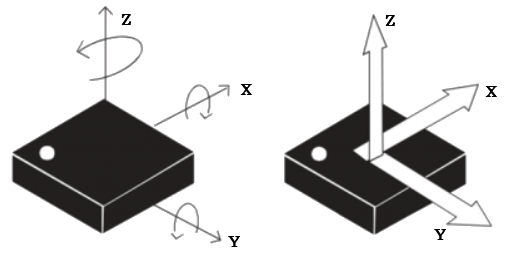
\includegraphics[scale=0.6]{figures/cDesign/LSM9DS1.png}
	\caption{På figuren ses akserne fra LSM9DS1. Til venstre ses magnometret, hvis akser er drejet én omgang i forhold til de to andre sensorer. I midten ses gyroskopet med sine roterende akser og til højre ses accelerometerets akser.\citep{Jimb02016}}
	\label{vores_IC}
\end{figure}

Sensoren besidder fire pins på sin venstre side, som vil blive benyttet i dette projekt. Disse kan ses på \figref{fig:IC_pins}. GND og VDD er jord og strømforsyningspins, mens SDA er I$^2$C datapin, hvor al data bliver sendt og modtaget igennem, og SCL er en seriel clock, der blandt andet sørger for synkron datasampling.
\begin{figure}[H]
	\centering
	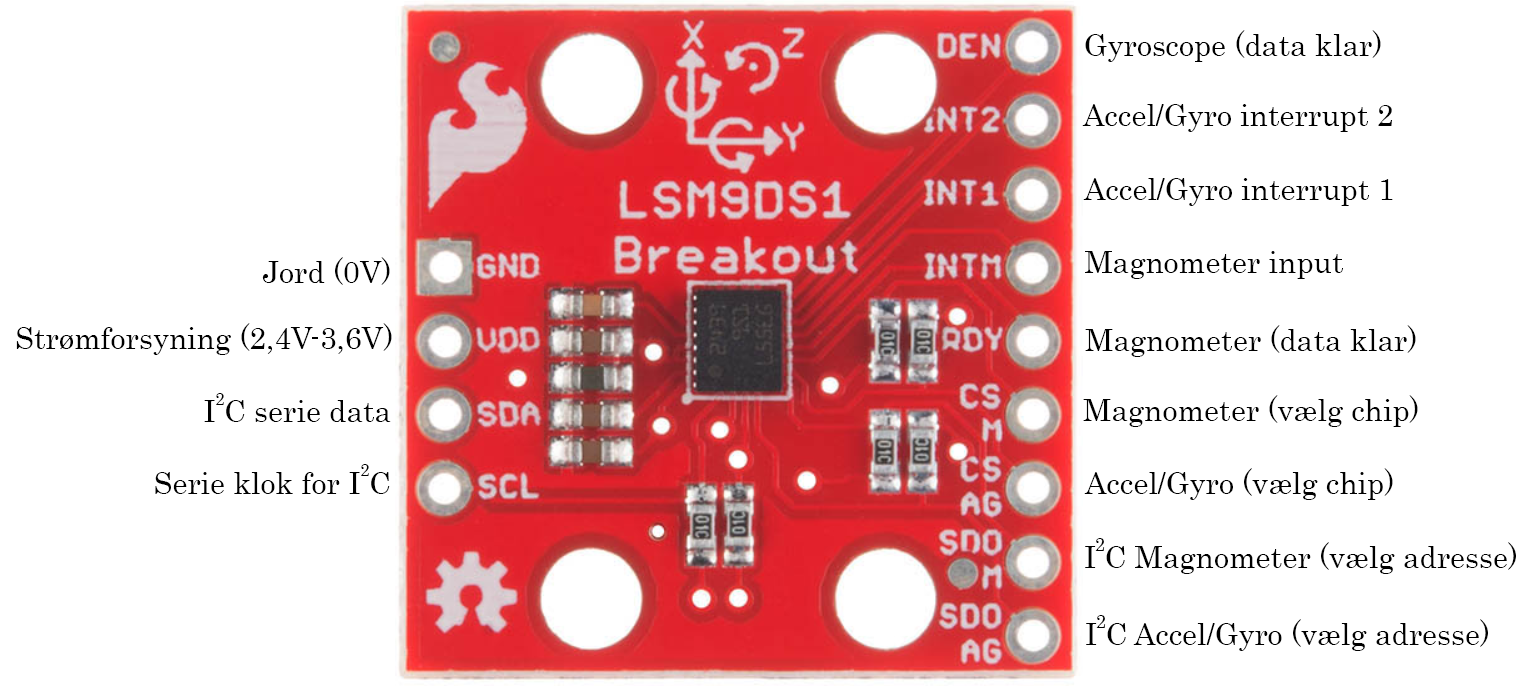
\includegraphics[scale=0.35]{figures/cDesign/accelerometeret.png}
	\caption{På figuren ses pinkonfigurationen af LSM9DS1. \citep{Jimb02016}}
	\label{fig:IC_pins}
\end{figure}
LSM9DS1 er en digital sensor, hvormed de analoge signaler konverteres til digitale i IC'en ved hjælp af en indbygget 16 bits ADC. Derfor skal sensoren indstilles til en bestemt samplingsfrekvens igennem algoritmedesignet til den. Ifølge \secref{sec:krav} skal accelerometret sample med mindst 450 Hz. Databladet informerer om, at accelerometret kan samples med seks værdier, hvoraf to steps er 238 eller 476 Hz. Derfor vælges samplingen for accelerometret til 476 Hz. Gyroskopet skal samples med mindst 60 Hz, men ifølge gyroskopets datablad kan den enten indstilles til 59,5 eller 119 Hz, hvorfor den indstilles til 119 Hz.

Det digitaliserede signal kan både bruges med en SPI og en I$^{2}$C styrefunktion, hvor mikrokontrolleren CY8CKIT-043 PSoC 4-M besidder begge. Der ønskes at benytte I$^{2}$C funktionen, da ICen dermed både skal sende og modtage data.\fxnote{Modtage om gyroskopet skal tændes eller slukkes.} For at gøre dette skal koden i algoritmedesignet benytte I$^2$C metoden til at skrive til et bestemt registor. På \figref{Fig:master_slave} ses kommunikationen mellem en master og slave, hvoraf slaven i dette tilfælde er ICen og masteren er MCUen.\fxnote{Og dette kan ikke vendes om, ICen vil ALTID være slaven} Der ses, at MCUen skriver en start kode til ICen for at starte kommunikationen. Herefter skriver masteren én bit til slaven, som skal godkende, at dette er modtaget. Så vil masteren give en adresse til slaven, som bestemmer hvorfra sensoren skal give data. Når slaven har godkendt dette, skriver masteren til slaven, at den gerne vil læse fra slaven, hvilket tillades og data hentes over på masteren. Afslutningsvist skriver masteren en stop kode til slaven, hvorefter kommunikationen er afbrudt. %For at benytte I$^{2}$C funktionen sættes pin CS\_AG høj, og de fire pins SDO og CS benyttes ikke. Alle pins kan ses på \figref{IC_pins}. Før et signal kan registreres kobles pinnen GND til jord, og på benet VDD skal der leveres mellem 1,9 V og 3,6 V.\fxnote{skriv resten af opsætningen efter at have snakket med John}. 
\begin{figure}[H]
	\centering
	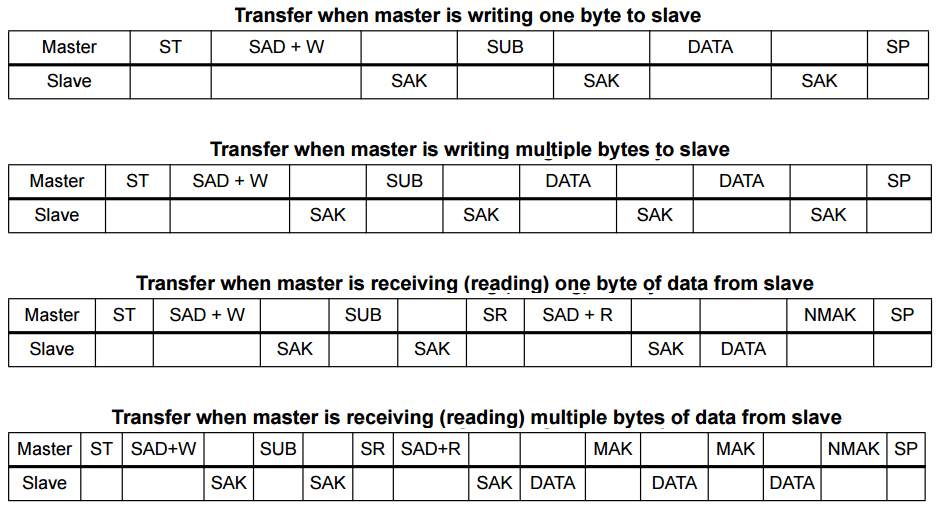
\includegraphics[scale=0.6]{figures/cDesign/Sensor_write_read.png}
	\caption{På figuren ses fire forskellige metoder for kommunikation imellem slave og master enhed, der afhænger af, om man vil henholdsvis læse eller skrive en eller flere bits.\citep{STMicroelectronics2016}}
	\label{Fig:master_slave}
\end{figure}
I LSM9DS1 forbruger gyroskopet 4 mA og accelerometeret 600 $\mu$A ved normale betingelser\fxnote{hvor Vdd er forsynet med 2,2V og temperaturen er 25 grader}. Det er derfor essentielt, at gyroskopet bruges så lidt som muligt, når systemet skal være batteridrevet og kun benytter accelerometret til datasampling. Det er muligt enten at slukke begge sensorer, at benytte accelerometeret alene eller benytte både accelerometeret og gyroskopet sammen, hvor begge har samme mængde output af data. Der kan yderligere spares strøm ved brug af gyroskopet, hvis der vælges en lavere samplerate.\\ % alt efter hvor hurtigt et signal skal samples. 
Gyroskopet har tre forskellige power modes: slukket, low power og normal power. For at gyroskopet kan være i low power, skal outputtet af data være på 14,9-119 Hz. Hvis outputsignalet er over dette, vil gyroskopet automatisk gå i normal power. Ifølge \secref{Sec:krav} skal gyroskopet samples med mindst 60 Hz, men samplingen kan enten være 59,5 eller 119, hvorfor den indstilles til 119 Hz. Derfor kan gyroskopet til dette projekt køre i low power mode. \citep{STMicroelectronics2016}
%Accelerometeret og gyroskopet har 32 åbninger af 16 bit data FIFO til hver af gyroskopets akser, samt 16 bit FIFO til hver af accelerometerets akser. Derved skal data ikke konstant sendes til en enhed og der kan spares strøm. Bufferen kan virke på fem forskellige måder, hvor der er tre overordnede tilstande: Bypass tilstand, FIFO tilstand og kontinuert tilstand, som alle tre er illustreret på \figref{tilstand}. Derudover er der to kombinerede tilstande: kontinuert-til-FIFO tilstand og bypass-til-kontinuert tilstand. \newline
%\begin{figure}[H]
%	\centering
%	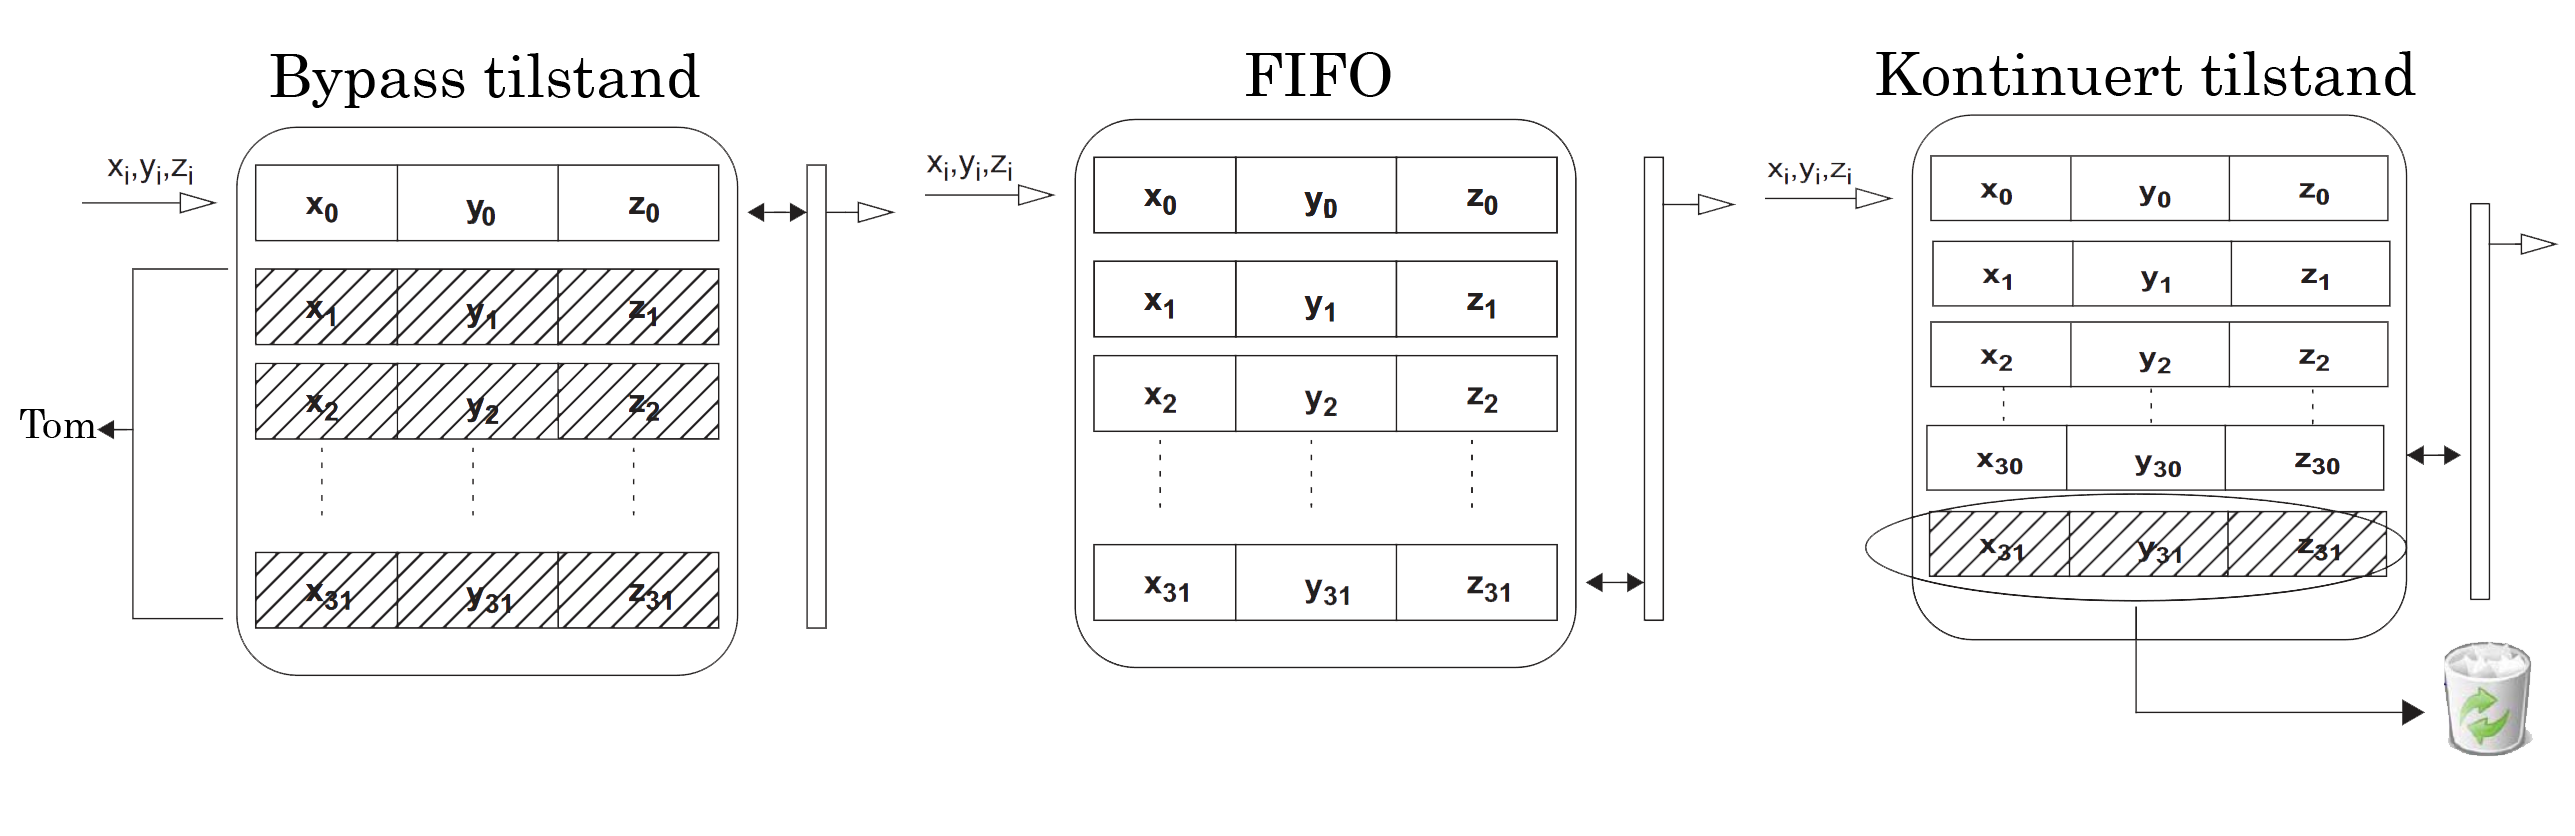
\includegraphics[scale=0.28]{figures/cDesign/LSM9DS1_tilstand.png}
%	\caption{På figuren ses de tre overordnede tilstande IC'en kan opsamle data med.\citep{Jimb02016}}
%	\label{tilstand}
%\end{figure}
%I bypass tilstanden bruges kun den første adresse, som overskrives når ny data er tilgængelig. Denne tilstand benyttes blandt andet til at nulstille FIFO
%FIFO stilstanden bruges til at lagre data i niveauer indtil ny data overskriver det gamle. Det er muligt at gemme data i 32 niveauer, men dette kan tilpasses mindre efter behov. For at gammel data ikke overskrides indsættes et interrupt når FIFO er fyldt, hvormed der ikke lagres ny data. 
%Den kontinuerte tilstand muliggør kontinuert FIFO, hvormed ny data overskriver gammel data. 
%Ved kontinuert-til-FIFO tilstand skifter tilstanden alt efter de bit der modtages i interruptet for accelerometeret og gyroskopet. Hvis der modtages et bit på 1 vil den være i FIFO tilstand, og modtages der et bit på 0, vil den være i kontinuert tilstand. 
%I bypass-til-kontinuert tilstand skiftes der ligeledes mellem bypass og kontinuert tilstand alt efter det modtagne interrups for accelerometeret og gyroskopet. Hvis der modtages et bit på 1, er den i kontinuert tilstand, og modtages der en bit på 0, nulstilles den ved at gå i bypass tilstand. 
\subsection{Implementering}





%Accelerometrets sensitivitet ved 16 g målinger: 0,732 mg/LSB
%Hvor LSB er 2*16/2^16 = 0.0078125
%(Man får et output på ca. 1350 fra acc, hvilket giver næsten 1 ganget med 0,732 mg/LSB)
%
%Gyroskopets sensitivitet med 2000 dps målinger: 70 mdps/LSB
%Hvor LSB er 2*2000/2^16 = 0.97656
%()

